% !TeX root = RJwrapper.tex
\title{The \pkg{HBV.IANIGLA} Hydrological Model}
\author{by Ezequiel Toum, Mariano H. Masiokas, Ricardo Villalba, Pierre Pitte and Lucas Ruiz}

\maketitle

\abstract{
Over the past 40 years, the HBV (Hydrologiska Byråns Vattenbalansavdelning) hydrological model has been one of the most used
worldwide due to its robustness, simplicity, and reliable results. Despite these advantages, the available versions impose some
limitations for research studies in mountain watersheds dominated by ice-snow melt runoff (i.e., no glacier module, a limited
number of elevation bands, among other constraints). Here we present HBV.IANIGLA, a tool for hydroclimatic studies in regions
with steep topography and/or cryospheric processes which provides a modular and extended implementation of the HBV model as 
an R package. To our knowledge, this is the first  modular version of the
original HBV model. This feature can be very useful for teaching hydrological modeling, as it offers the possibility to
build a customized, open-source model that can be adjusted to different requirements of students and users.}


\section{Introduction}

Hydrological modeling is widely used by engineers, meteorologists, geographers, geologists, and researchers interested in knowing
the runoff of rivers in the coming days or the variations of the snowpack under certain temperature or precipitation changes, 
among many other hydrological processes.\\
The Swedish Meteorological and Hydrological Institute (SMHI) ran the first successful simulation of the HBV model in 1972.
It was developed to forecast river runoff for hydropower generation in Sweden \citep{bergstrom:2015}. Up to now,
many versions have been developed: HBV-ETH (Switzerland - \citet{braun:1992} ), HBV-Light (Switzerland - \citet{seibert:2012} ), 
HBV-D (Germany - \citet{krysanova:1999} ), HBV-CE (Canada - \citet{stahl_hbv:2008} ), \CRANpkg{TUWmodel}
(Austria - \citet{viglione:2016} ), among others. Despite all these free versions, none of them allows the users 
to build their own model using a self-defined combination of modules.


\citet{buytaert:2008} identified some prerequisites for hydrological model development: (1) \emph{accessibility} in order to
reproduce experimental results; (2) \emph{modularity} as a key element for the development of new \emph{‘ad-hoc’} models
to evaluate several aspects of the hydrological cycle and to propose improvements; (3) \emph{portability}, so the model can run
in many operating systems; and (4) \emph{open-source code} as a fundamental scientific requirement that allows users to revise,
correct, and suggest code improvements.

\citet{slater:2019} highlighted some of the key R packages for hydrological modeling; \pkg{TUWmodel} is an R version of the HBV
model originally written in Fortran \citep{viglione:2016}; \CRANpkg{topmodel} and \CRANpkg{dynatopmodel} are the R versions of
the well-known semi-distributed models TOPMODEL and Dynamic TOPMODEL \citep{topmodel:2018, metcalfe:2015}; \CRANpkg{airGR} 
\citep{coron:2017, airGR:2020} includes several conceptual rainfall-runoff models, a snow accumulation and melt model and
the associated functions for their calibration and evaluation; finally, \pkg{hydromad} \citep{andrews:2011} provides a 
modeling framework for environmental hydrology through water balance accounting and flow routing in spatially aggregated
catchments.

Of the models mentioned above, only \pkg{airGR}, \pkg{hydromad}, and \pkg{TUWmodel} present a snow routine to account for
accumulation and melting processes (temperature index model), but none of them have routines to account for glacier mass
balance. On the other hand, the \CRANpkg{glacierSMBM} package \citep{glacier:2017} allows the modeling of glacier surface mass
balance in a fully distributed manner, but it was designed to work on the mass balance of a single glacier and to run on a 
raster-based grid, two aspects that limit its applicability at the basin scale.

The \CRANpkg{HBV.IANIGLA} \citep{toum:2021} package was built with the aim of providing a modular hydrological model 
approach that adds to the classic HBV routines functions for the modeling of the surface mass balance of clean and 
debris-covered glaciers, a fundamental aspect in the hydrological cycle of  cold regions of the Andes \citep{masiokas:2020}. 
The main objective of this article is to present the \pkg{HBV.IANIGLA} model structure through its implementation as an
R package to serve as a practical guide to better understand how it works. The paper is organized as follows:

\begin{itemize}
	\item In the next section, we describe the modeling philosophy under HBV and justify the use of a modular approach. 
	We then present the \pkg{HBV.IANIGLA} modules and related equations (with some conceptual drawings).
	We end this section with a small study on model computation times, a fundamental aspect for sensitivity and 
	uncertainty analysis.
	\item Following the methodology, we focus on two examples: on a synthetic basin and on glacier mass balance.  
	The reader will find more reproducible examples in the package vignettes.
	\item Finally, we condense the key points of the current version of \pkg{HBV.IANIGLA} and propose future improvements.
\end{itemize}

\section{The HBV.IANIGLA model}

\subsection{The HBV model}

The HBV model has been used for $40$ years for hydrological studies in mountain 
regions around the world \citep{bergstrom:2015}. The model requires relatively few data inputs (air temperature,
precipitation, and potential evapotranspiration),  which makes it very appropriate in scarce data regions such
as the Southern Andes. It has been well-documented by other authors \citep{seibert:2012, parajka:2008, stahl_hbv:2008}, 
a feature that facilitates writing new codes and modifying or improving existing equations. Also	, it is a bucket-type 
model with relatively few free parameters to calibrate. 

The \pkg{HBV.IANIGLA} version not only takes into account precipitation phase partitioning, snow accumulation and melting, actual
evaporation and streamflow discharge, but also incorporates a module for simulating the surface mass balance of clean and 
debris-covered glaciers and another module for glacier-melt routing. In addition, the package has been designed in a modular
fashion, allowing users to build their own model. To our knowledge, this is the first HBV version and R hydro-modeling package 
to combine these two features.


\subsection{General modeling philosophy}

According to \citet{bergstrom:2015}, the HBV model was inspired in the works developed in the early 1970s by
\citet{nash:1970}, \citet{oconnell:1970}, and \citet{mandeville:1970}. The primary objective of this model was operational: to
forecast streamflow discharge for the Swedish hydropower industry. This overriding requirement dictated the characteristics of the
model: it should not be too complex but physically sound; the input data should conform to standard Swedish meteorological
measurements; the number of free parameters should be kept to a minimum; and it should be easy to understand.

The above features and lessons learned over more than two decades \citep{bergstrom:1991} resulted in a hydrological model
composed of four modules: ($1$) a temperature index model with an air temperature-based precipitation partitioning algorithm;
($2$) a soil moisture routine with a nonlinear empirical algorithm to account for abstractions, actual evaporation, and antecedent
conditions; ($3$) a bucket-type model (many variants exist up to now) to simulate the catchment storage effect; and ($4$) a transfer function to adjust the timing of the hydrograph to
the observed discharge.

To date, the model has not only been used in operational hydrology but also in scientific research.
\citet{konz:2010} used the HBV-Light version in three alpine catchments in Switzerland and Austria to show the value of glacier
mass balances in constraining uncertainty in the parameter estimation of conceptual models such as HBV. \citet{ali:2018} also applied
HBV-Light to evaluate model performance in a climate change context in the snow- and ice-dominated Hunza River basin in the
Karakoram Mountains, Pakistan. \citet{finger:2015} compared model performance in simulations of increasing complexity for glacier
mass balance and streamflow at the outflow of three Swiss watersheds. \citet{stahl_hbv:2008} used HBV-CE to estimate streamflow
sensitivity to different climate change scenarios in British Columbia, Canada. \citet{staudinger:2017} studied the variation of 
water storage with elevation in $21$ Swiss alpine and pre-alpine catchments using four different methods: water balance analysis, 
flow recession analysis, calibration of the HBV model, and calibration of a transfer function hydrograph separation model using 
stable isotope observations. In another interesting application, \citet{ren:2018} combined HBV with a Bayesian neural network to 
improve seasonal water supply forecasting in the Yarkant River basin, Central Asia. Therefore, the original conception of HBV and 
its evolution have made it a longstanding multipurpose tool for a diverse and dynamic user community.


\subsection{Modules and equations}

Models are based on a perceptual conception of the basin's functioning. This perception leads to the decision of the equations 
(hydrological processes) and the construction of a conceptual model \citep{beven:2012}. In the \pkg{HBV.IANIGLA} model, these first
two stages have already been decided, as the equations and coding are in the package, but the user still has a choice on how the
watershed or glacier will be discretized (in terms of land use and spatial aggregation) and on how the different modules will be
assembled. This decision should be guided by the objective of the project, the knowledge of the hydrological driving
process at the chosen modeling scale, and the data available not only for the implementation but also for the model
evaluation.


\begin{figure}[htbp]
  \centering
  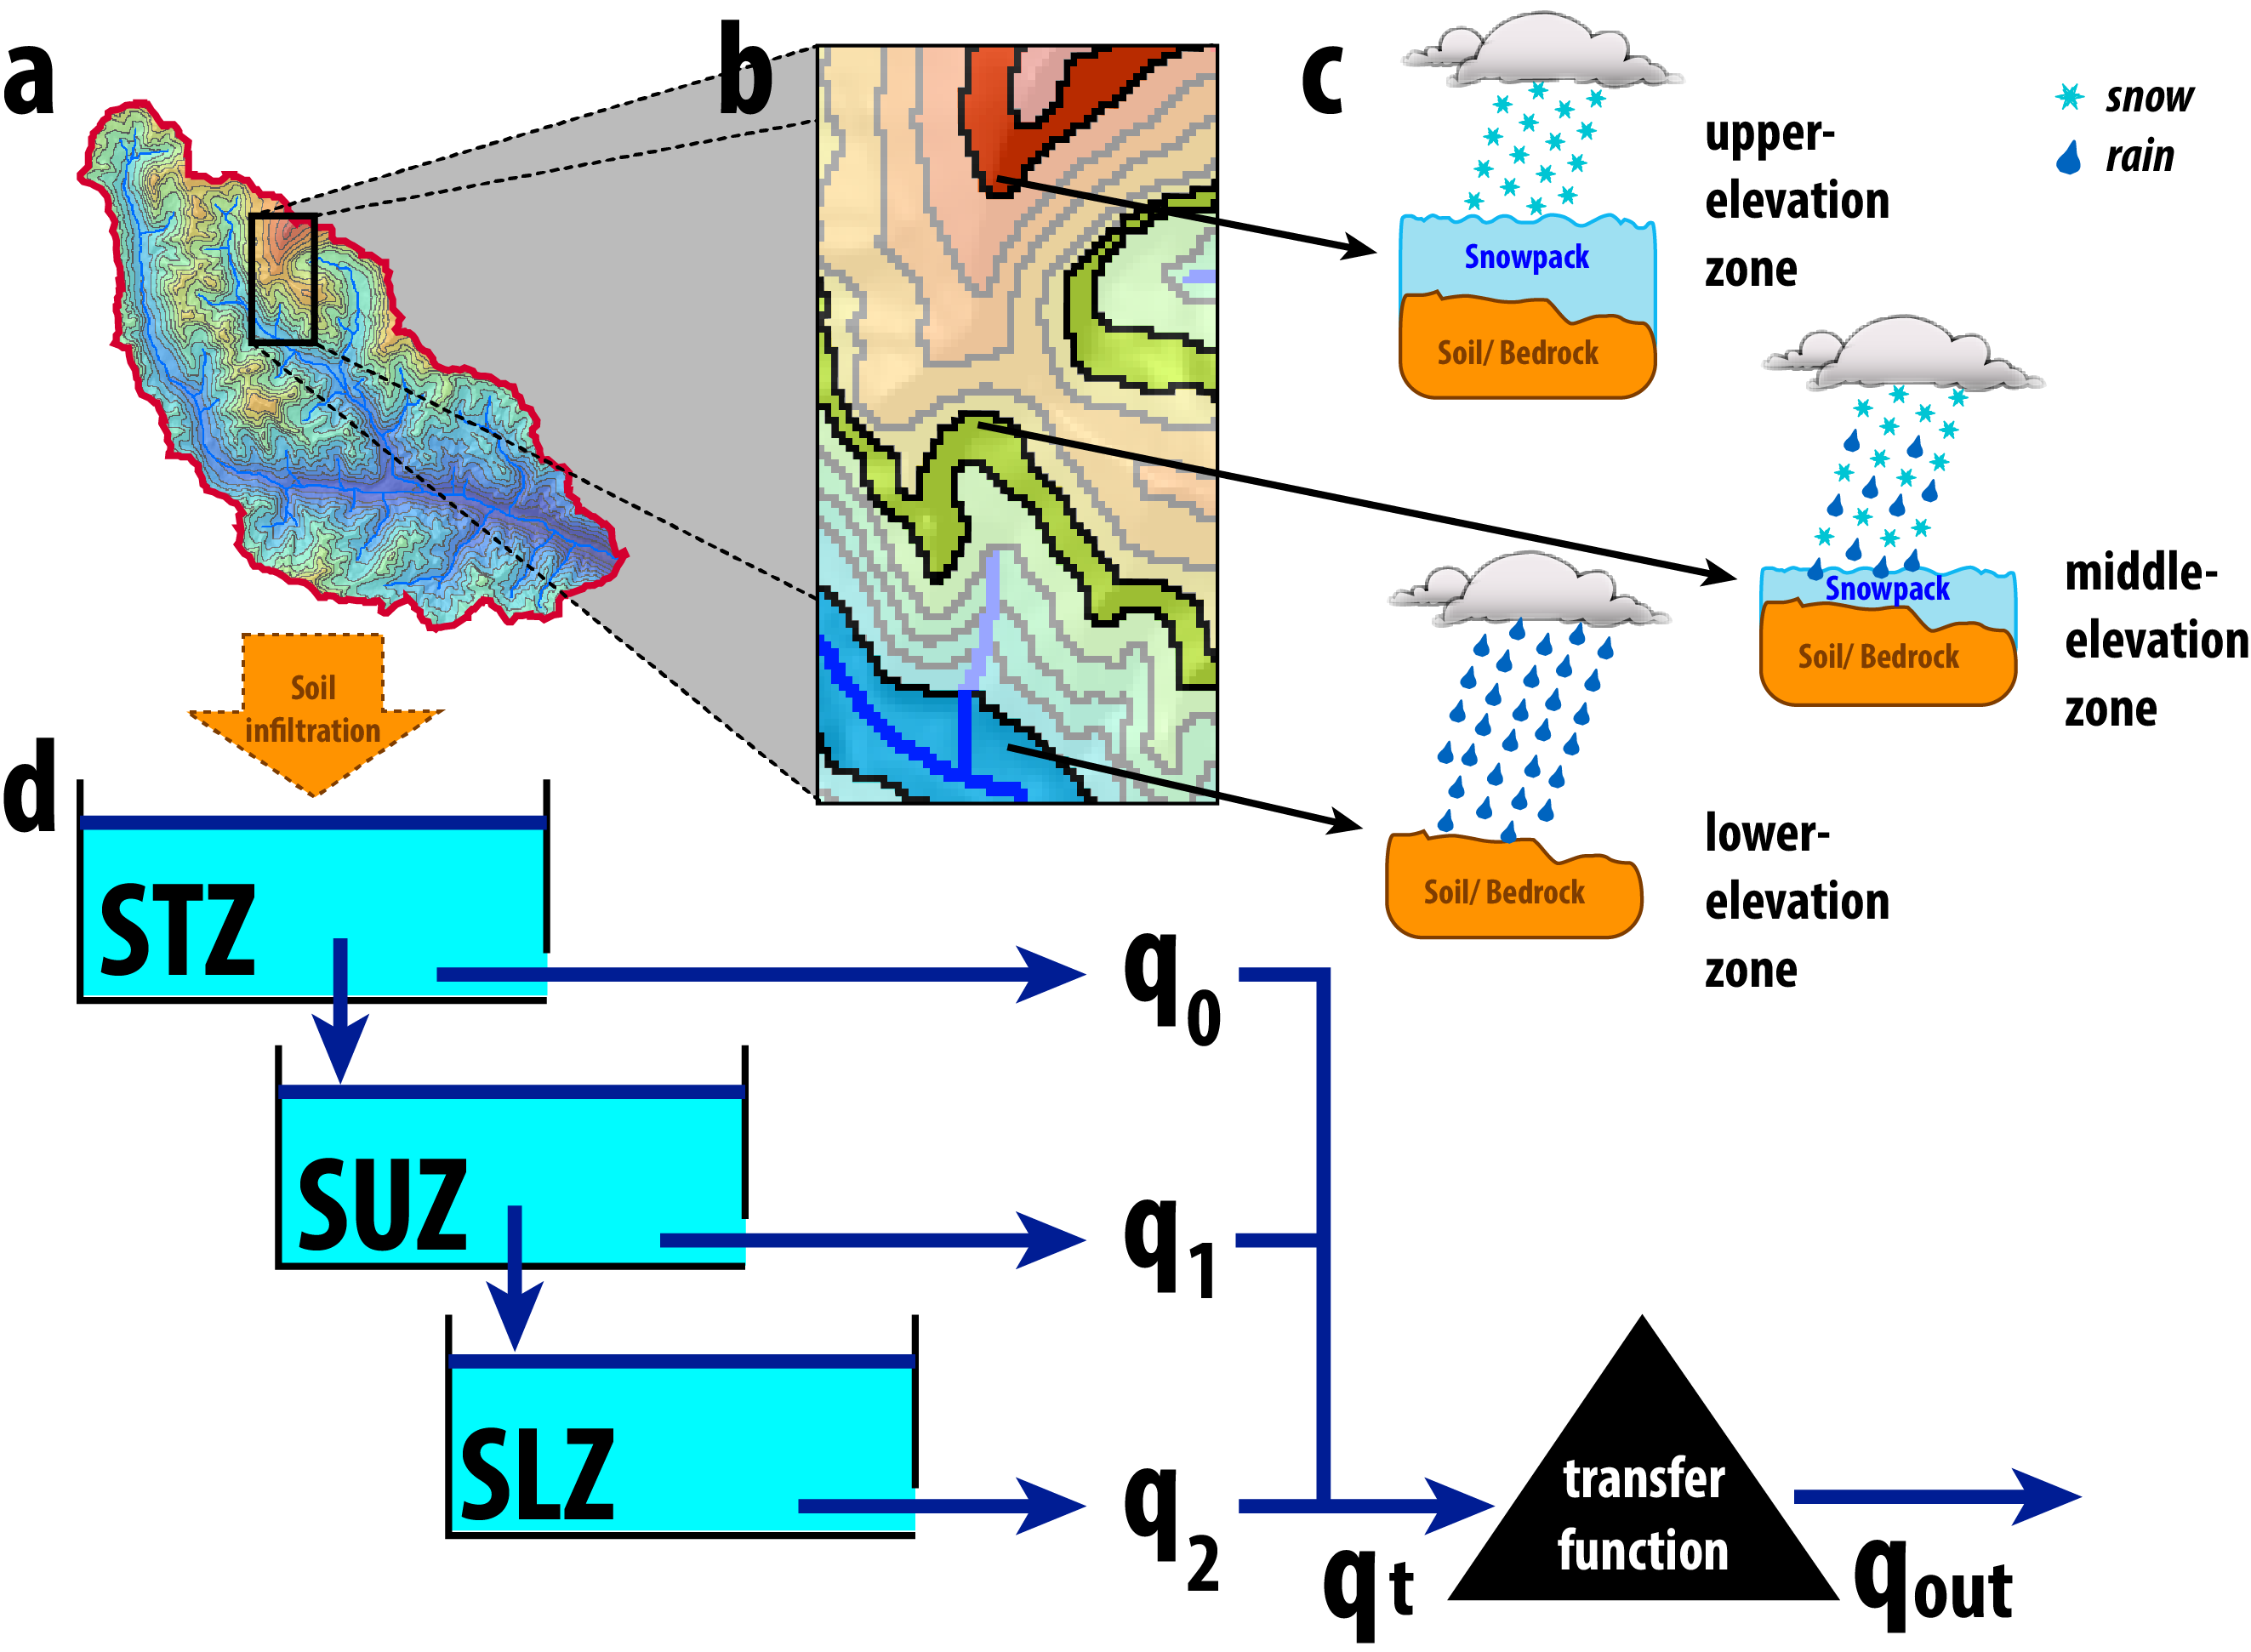
\includegraphics[scale = 0.6]{basin_hbv_2}
  \caption{Example of \pkg{HBV.IANIGLA} module assembly in a mountain basin. To account for snow accumulation and snowmelt, the
  basin has been discretized into elevation bands (\textbf{a} and \textbf{b}). Each of these polygons has snow and soil routine
  (\textbf{c}), the effective soil recharge, weighted according to the relative area of the elevation band, is passed to the bucket
  model (\textbf{d}). Finally, the river runoff timing is adjusted by a triangular transfer function.}
  \label{figure:basin_hbv}
\end{figure}

The following lines describe the modules that must be assembled to build a complete \pkg{HBV.IANIGLA} hydrological model. 
There are three other functions within the package: \code{PET}, \code{Pecip{\_}model}, and
\code{Temp{\_} model}. The first function contains a potential evapotranspiration model that provides a simple and 
straightforward way to calculate one of the inputs to the soil routine. However, for real-world applications we strongly
recommend the use of the specialized \CRANpkg{Evapotranspiration} package \citep{pet:2020}. The other two functions are linear
models to extrapolate air temperature and precipitation records. Since we consider that their use is straightforward, 
we refer the user to the package manual.


\subsubsection{Snow and ice melt models – \code{SnowGlacier{\_}HBV()}}

Precipitation is considered to be either snow or rain, depending on whether the temperature is above or below a threshold
temperature \textit{Tr} (ºC). 

\begin{align}
\begin{aligned}
P_{rain} & = P \quad         & \textit{if} \quad T_{air} > Tr \\
P_{snow} & = P * SFCF \quad  & \textit{if} \quad T_{air} \leq Tr
\end{aligned}
\end{align}

\noindent
After partitioning, the snowfall is corrected using the \code{SFCF} parameter to account for the under-capture effect of the 
precipitation gauge on snow events.

This function uses a temperature index approach for snow and glacier melt simulation. This kind of approximation has been widely
used in snow hydrology and glaciology, and different formulations have emerged 
\citep{hock:2003, seibert:2012, braun:1992}. The temperature index formulation takes into account the strong correlation between
snow line retreat and accumulated temperatures above a certain threshold (with typical values around $0$ºC). Hence although many
authors have proposed more complex formulations (e.g., HBV-Light uses a refreezing and liquid retention factor) or even a radiation
term \citep{pellicciotti:2005}, this empirical formulation must be parsimonious to avoid problems of overparameterization 
\citep{kirchner:2006}.

\begin{align}\label{eq:t_ind}
& Melt = (T_{air} - Tt) * f_{x} \quad \quad \textit{if} \quad T_{air} > Tt ,
\end{align}

\noindent
where $T_{air}$ is the measured or estimated air temperature, $Tt$ is the melting temperature, and $f_{x}$ is a generic expression
of melting factors for snow, clean, or debris-covered ice.

If the air temperature is above the threshold ($Tt$), melting occurs at a rate proportional to the melting factor ($f_{x}$). Both
the temperature threshold and the melting factor are parameters that must be calibrated by the user. Note that the time units
depend on the resolution of the input data. Although the examples shown in this article are in a daily time step, the model can
be used in the hourly or monthly resolution. In the next lines, we will describe in detail the different arguments of the
function.

The \code{model} argument presents three options:

\begin{enumerate}
	\item \textbf{Temperature index model}: this model is described by equation \ref{eq:t_ind}. Here, the user can apply
	the most common and recommended set of temperature index formulations.
	\item \textbf{Temperature index model with variable snow cover area}: this option is an attempt to offer, within the package,
	the same temperature index model as in the Snowmelt Runoff Model \citep{dewalle:2008}. However, this routine has certain
	limitation: the snow cover series forces the model to simulate a total effective value (e.g., snow water equivalent), which
	is not in-line with the original idea of modeling in elevation bands, where average values are expected. 
	\item \textbf{Temperature index model with a variable glacier area}: this routine explicitly takes into account the 
	change in glacier area. Since the automatic reduction of glacier area forces the simulation to the observed values,
	the user should evaluate the correspondence between the simulated and observed mass balances.
\end{enumerate}

The package documentation contains all the necessary information (vignettes with reproducible examples included) to 
correctly construct the \code{inputData} argument. The data matrix must not contain missing values (\code{NA's}) because
\pkg{HBV.IANIGLA} is a continuous hydrological model, meaning that it simulates all the variables in every time step.

The initial conditions of the model are (\code{initCond}):

\begin{enumerate}
	\item \textbf{Initial snow water equivalent}: this is a state variable, whose initial value will be used in the first loop. Unless
	field data is available, it is recommended to use a zero value. Because uncertainties are common in the initial state 
	variables of the model, it is recommended to use a warm-up period (between one and two years in daily time step modeling).
	If the period covered by the data is very limited, these same values can be used as calibration parameters.
	\item \textbf{Numeric integer indicating the surface type}: 1: clean ice; 2: soil; 3: debris-covered ice. \pkg{HBV.IANIGLA}
    uses this argument to know which parameters (\code{param} argument) to look for. It also constrains the function output. 
	\item \textbf{Area of the glacier(s) (in the elevation band) relative to the basin}:  this is required only if the surface
	 is a clean or debris-covered glacier. The area is used to scale the total amount of water produced (rainfall plus melted
	 water) according to the area of the polygon in the basin. Thus, if the area of this portion of the glacier corresponds to 5\%
	 of the basin area, a value of $0.05$ should be assigned.
\end{enumerate}

The last argument is a numeric vector that stores the parameter values (\code{param}) of the modules. For debris-covered glaciers,
a dummy value for the clean glacier melting factor (\code{$f_{ic}$}) must be supplied. This value will not be used internally 
but simplifies the calibration exercise when working in a basin with both types of glaciers.

It should be noted that this function allows the construction of a single and lumped simulation. In order to develop the model 
for the example shown in figure \ref{figure:basin_hbv}, it will be necessary to build the model by running the function once per
every elevation band (see examples in \code{vignette(package = "HBV.IANIGLA")}).


\subsubsection{Soil routine – \code{Soil{\_}HBV()}}

This routine is based on an empirical formulation that takes into account actual evapotranspiration, antecedent conditions,
and effective soil infiltration. This relationship is described by the so-called beta function \citep{bergstrom:2015}, 

\begin{align}
& Inf = (Melt + Rainfall) * \left( \frac{SM}{FC} \right)^\beta ,
\end{align}

\noindent
where $Inf$ is the soil box infiltration, $SM$ is the soil moisture state variable, and 
$\beta$ is a nonlinear parameter between the total amount of water entering the soil box, soil moisture storage, and runoff
generation. This equation is not unique among bucket-type hydrological models. A similar formulation can be found  in the 
VIC model \citep{liang:1994}. \pkg{HBV.IANIGLA} assumes that all evapotranspiration occurs from the soil box, so this function 
implicitly accounts for all abstractions:

\begin{align}
& E_{act} = E_{pot} * min \left( \frac{SM}{FC * LP}; 1.00 \right) ,
\end{align}

\noindent
where $E_{act}$ is the actual evapotranspiration, $E_{pot}$ is the potential evapotranspiration, $FC$ is the soil box water 
capacity parameter, and $LP$ is a reduction factor. 

This type of relationship between potential, actual evapotranspiration, and soil moisture content has been
found by \citet{zhang:2003} in eastern Asia, suggesting that despite its empirical formulation, in some places, it could
have some physical meaning. Finally, and similar to the snow and ice melt modules, this routine represents a single
and lumped simulation.

\subsubsection{Routine module – \code{Routing{\_}HBV()}}

After infiltration, the water follows several complex pathways to streams \citep{mcdonnell:2003}. A detailed description
and modeling of these water pathways requires field data and measurements that are generally not available. An early 
engineering-based solution to this issue was to consider this multi-causal delay as a water storage effect at the
catchment scale \citep{dooge:1973}. This practical modeling approach could be seen as series of linearly interconnected and
interrelated reservoirs \citep{sivapalan:2017}.

The current \pkg{HBV.IANIGLA} (version 0.2.1) has five different bucket formulations, which are selected by changing the model 
argument number (figure \ref{fig:bucket_models}). To solve the time step change in the bucket water storage,
we used the explicit finite difference form of the mass balance equation over a discrete-time step \citep{beven:2012}.
Although the general solution has been implemented for a single linear reservoir (figure \ref{fig:discrete}), we provide solutions
for the five-bucket models.

\begin{figure}[htbp]
     \centering
     \begin{subfigure}[b]{0.45\textwidth}
         \centering
         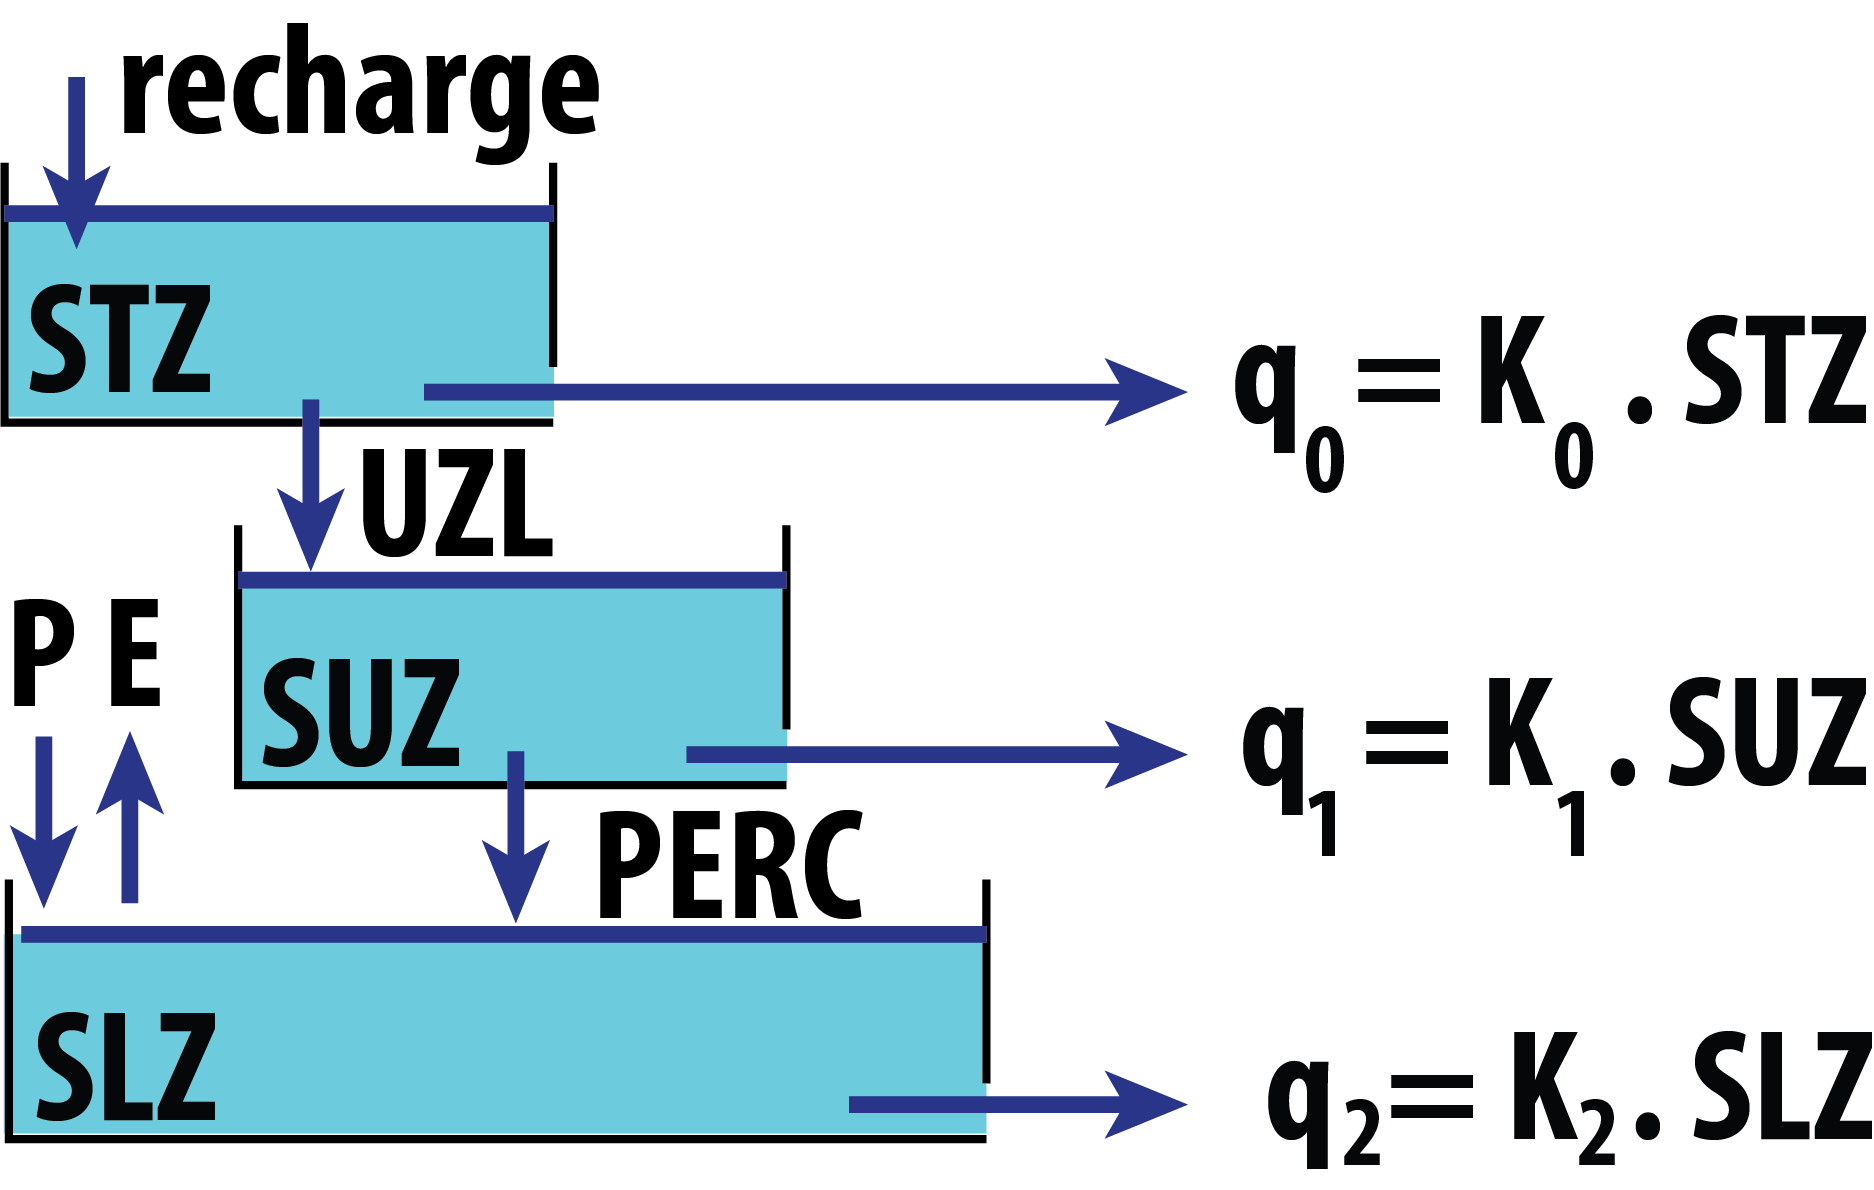
\includegraphics[width=\textwidth]{bucket_3_outlet_3}
         \caption{Model 1}
         \label{fig:b3_o3}
     \end{subfigure}
     \hfill
     \begin{subfigure}[b]{0.45\textwidth}
         \centering
         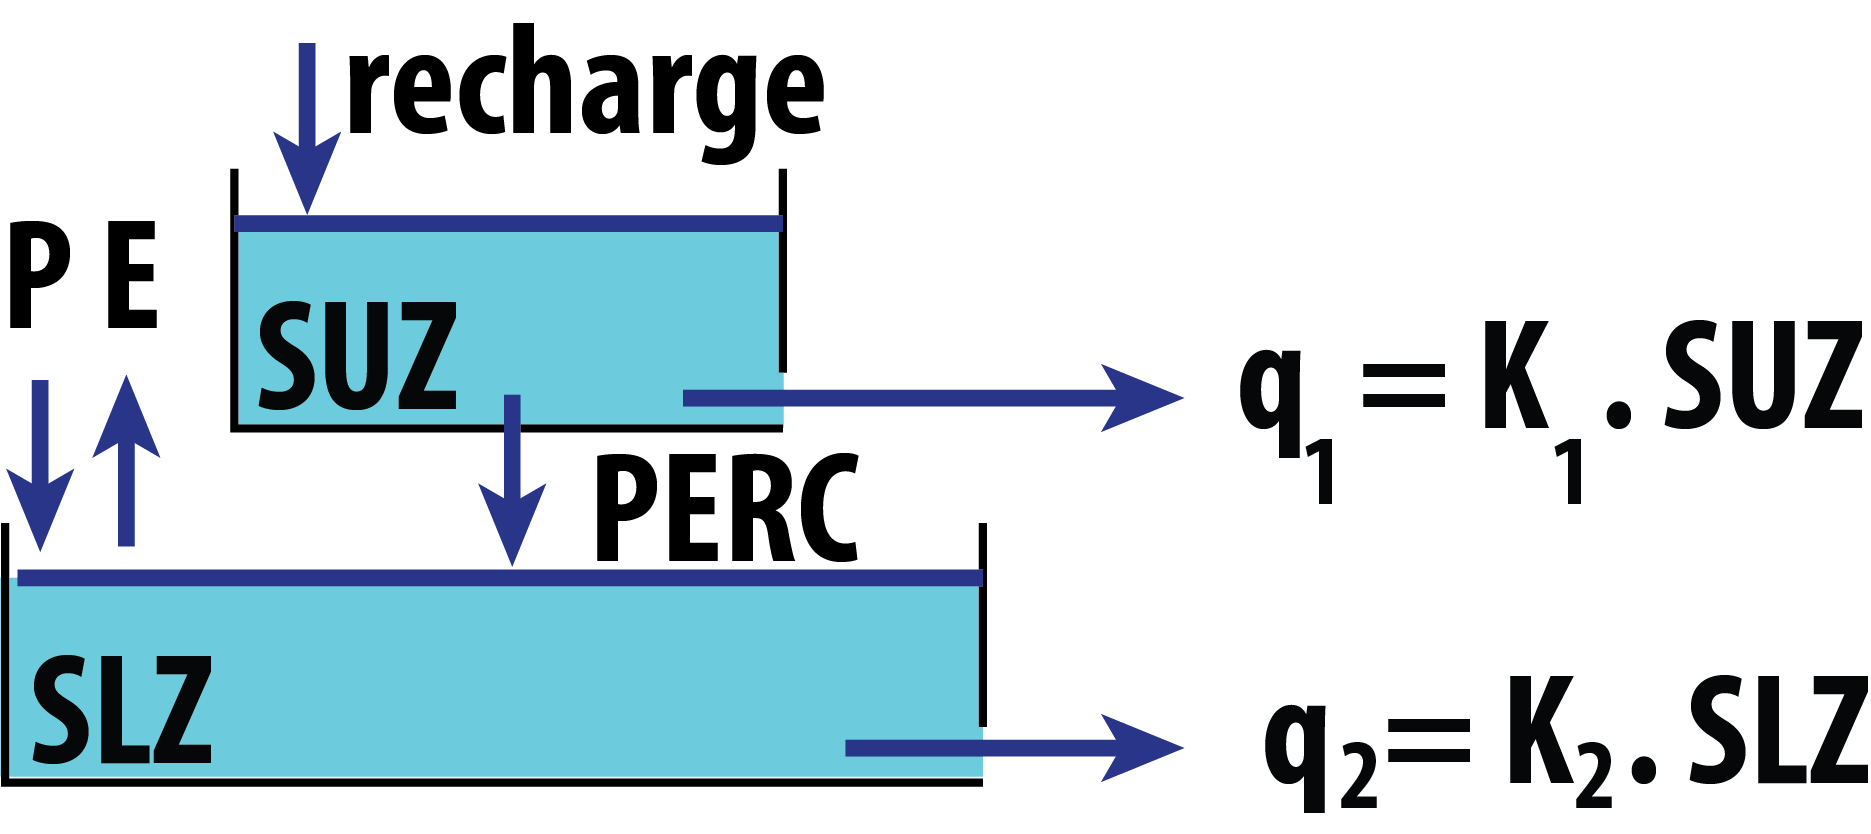
\includegraphics[width=\textwidth]{bucket_2_outlet_2}
         \caption{Model 2}
         \label{fig:b2_o2}         
     \end{subfigure}
     \caption{Diagrams for two of the five available bucket models. The reader will find all the diagrams in
     the help menu (\code{?Routing{\_}HBV}).}
        \label{fig:bucket_models}         
\end{figure}


\begin{figure}[htbp]
  \centering
  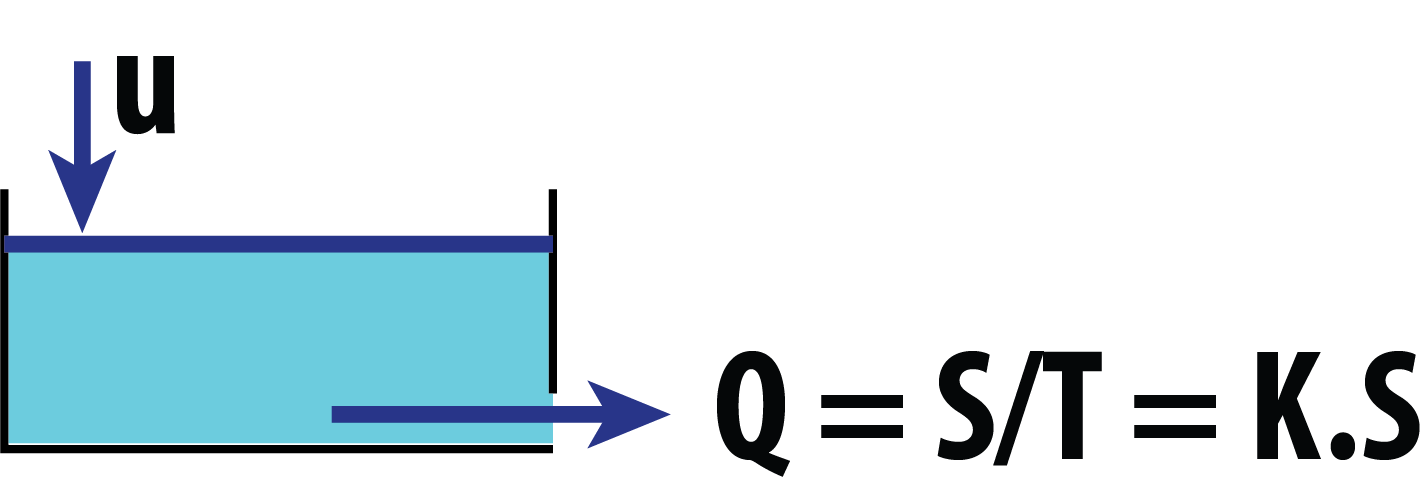
\includegraphics[scale = 0.6]{bucket_discrete_scheme}
  \caption{General outline for a water reservoir.}
  \label{fig:discrete}
\end{figure}

\begin{align}
& \frac{dS}{dt} = u - Q  \quad \quad \textit{mass balance equation} \\
& Q = K * S \quad \quad \quad \textit{continuity equation} \\ 
& \textit{from (6),} \nonumber \\
& S = \frac{Q}{K} = T * Q \\
& \textit{we replace (7) into (5),} \nonumber \\
& T * \frac{dQ}{dt} = u * Q \nonumber 
\end{align}

\noindent
In discrete time steps, we use the explicit finite difference form,

\begin{align}
& \frac{Q_t - Q_{t-\Delta t}}{\Delta t} = \frac{u_t - Q_{t-\Delta t}}{T} \nonumber \\
& Q_t = \frac{\Delta t}{T} * u_t + (1 - \frac{\Delta t}{T}) * Q_{t-\Delta t} \nonumber \\
& a = (1 - \frac{\Delta t}{T}) \nonumber \\
& b = \frac{\Delta t}{T} \nonumber \\ 
& Q_t = a * Q_{t-\Delta t} + b * u_t  \\
& \frac{S_t - S_{t-\Delta t}}{\Delta t} = u_t - Q_{t-\Delta t} \nonumber \\
& S_t = S_{t-\Delta t} + \Delta t * (u_t - Q_{t-\Delta t})
\end{align}

\subsubsection{Glacier routine module – \code{Glacier{\_}Disch()}}

Following an approach similar to previous routines, we adopt bucket storage and release scheme
\citep{jansson:2003}. In \pkg{HBV.IANIGLA}, we use the approach proposed by \citet{stahl_hbv:2008} for the HBV-EC model,
employed to estimate glacier and streamflow responses to future climate scenarios in the Bridge River Basin (British Columbia,
Canada). The glacier outflow is calculated as:

\begin{figure}[htbp]
  \centering
  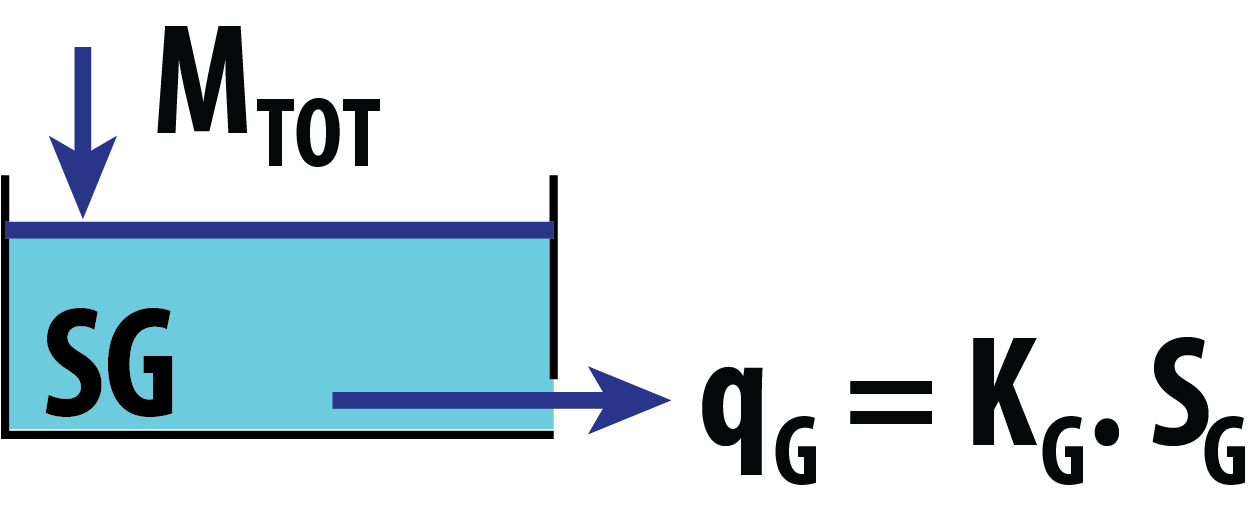
\includegraphics[scale = 0.6]{glacier_discharge_hbv}
  \caption{The glacier runoff release (precipitation plus snow and ice melt) is modeled as a linear water reservoir
  with a variable storage coefficient ($K_G$), which is a function of the snow water equivalent above the ice body.}
  \label{fig:glacier}
\end{figure}

\begin{align}
& K_G = K_{Gmin} + dK_G * \exp \left( SWE/AG \right) \\
& q_G = K_G * S_G ,
\end{align}

\noindent
where $K_{G}$ is the actual glacier outflow coefficient, $K_{Gmin}$ a minimum storage release coefficient, $dK_{G}$ the 
maximum glacier outflow increment, $SWE$ the total snow water equivalent over the glacier, $AG$ a scaling parameter, 
$S_G$ the glacier water storage, and $q_G$ the glacier runoff. 

Note that the storage coefficient is a function of a minimum coefficient (denoting poor drainage conditions on the glacier),
the snow water equivalent, and a calibration parameter. When the snowpack is at its maximum value, drainage occurs at 
a minimum rate, the opposite occurs in the late summer when all the snow on the glacier has melted. 

For the resolution of the time step change, we also use the explicit finite difference formulation of the mass balance equation.

\subsubsection{Transfer Function – \code{UH()}}

To represent the runoff routing in streams, we provide a single parameter triangular function. This parameter is calibrated 
to adjust the timing of the simulated river discharge,

\begin{align}
& Q = \sum_{i=1}^{B_{max}} Q_{t-i+1} * b_i ,
\end{align}

\noindent
where $B_{max}$ is the base of the triangular weighting function, $b_i$ is the weight for the $i^{th}$ step, and $Q_{t-i+1}$
is the sum of the glacier and soil bucket runoff.  

\subsection{Computation times}

The \pkg{HBV.IANIGLA} functions were written using \CRANpkg{Rcpp} \citep{eddelbuettel:2013, rcpp:2019}, a package
that extends the R language using C++. This approach combines the speed and efficiency of C++, a compiled language, with the
powerful interactive environment of R (see table \ref{table:performance}), a language where it is easy to implement specific
hydrological workflows (from data retrieval to results analysis) in a single environment
\citep{slater:2019}. 

\begin{table}[h!]
	\begin{tabular}{ c  c  c  c  c  c }
	\toprule
	\textbf{min} &  \textbf{lq} & \textbf{mean} & \textbf{median} & \textbf{uq} & \textbf{max} \\
	\midrule
	$1.79$       &   $1.95$     &   $2.65$      &     $2.01$      &   $2.19$    &  $55.81$ \\
	\bottomrule
    \end{tabular}
    \captionof{table}{Summary of computation times (in \textit{milliseconds}) over $1000$ runs of the \code{glacier{\_}hbv}
    function (see \code{vignette("alerce{\_}mass{\_}balance")}) . The glacier was discretized into $8$ elevation bands 
    ($\sim 100$ m range). The model was built with the modules \code{Temp{\_}model}, \code{Precip{\_}model}, and
    \code{SnowGlacier} and was run on a daily time step over a period of almost $9$ years (from 2010-01-01 to 2018-05-30).
    The analysis was performed on a CPU with an Intel Core i7-4790 processor at 3.60GHz, on a 64-bit OS running 
    Ubuntu 18.04 using the \CRANpkg{microbechmark} package \citep{microbench:2019}.}
    \label{table:performance}
\end{table}

Speed is an important issue for hydrological models, as it allows the user to perform not only uncertainty and 
sensitivity analysis in reasonable times, but also to apply demanding optimization algorithms such 
as \CRANpkg{DEoptim} \citep{de_opt:2016} or different model structures. This is a recommended practice in the field of 
hydrological modeling \citep{beven_manifesto_2006, beven:2008, pianosi:2016}. In addition, the package only depends on \pkg{Rcpp}
(v 0.12.0), a fact that supports its long-term maintenance. \\
If the reader is interested in comparing the computation times of different R hydrological models we recommend the work 
of \citet{paul:2020}.  


\section{Case studies}

\subsection{Lumped synthetic catchment}

As a first attempt at applying \pkg{HBV.IANIGLA}, a synthetic lumped catchment (the simplest hydrological model) is used to
introduce the construction of the model and to present a basin discharge calibration exercise.

Initially, the dataset containing: date, air temperature, precipitation, potential evapotranspiration, and the catchment outflow
is loaded, and then the model construction is conducted (from top to bottom).

\begin{example}
library(HBV.IANIGLA)

# load the lumped catchment dataset
data("lumped_hbv")

# take a look at our dataset
head(lumped_hbv)
summary(lumped_hbv)
\end{example}

For a basin without glaciers,  the \code{SnowGlacier} module is used only with soil as the underlying surface. 
In this exercise, we provide the correct initial conditions and parameters for all modules except the \code{Routing{\_}HBV}
function. Consistent with the development of hydrologic models, we build our model in a top-down direction, 
from precipitation to streamflow routing (note that most hydrological books are structured in the same way).

\begin{example}
# consider the SnowGlacier module to take into account 
# precipitation partitioning and the snow accumulation/melting. 
snow_module <-
  SnowGlacier_HBV(model = 1, 
                  inputData = as.matrix( lumped_hbv[ , c(2, 3)] ),
                  initCond = c(20, 2), 
                  param = c(1.20, 1.00, 0.00, 2.5) )
                  
# now pass rainfall plus snowmelt to 
# the soil routine. Note that we are using the PET series,                 

soil_module <-
  Soil_HBV(model = 1,
           inputData = cbind(snow_module[ , "Total"], lumped_hbv[ , "PET(mm/d)"]),
           initCond = c(100, 1),
           param = c(200, 0.8, 1.15) ) 
\end{example}

The actual evapotranspiration, soil moisture, and recharge series are obtained from the last module. Subsequently, the recharge is
incorporated into the routing function. Recall that the routing parameters (\code{param} argument) are not calibrated.

\begin{example}
routing_module <-
  Routing_HBV(model = 1, 
              lake = F, 
              inputData = as.matrix(soil_module[ , "Rech"]),
              initCond = c(0, 0, 0), 
              param = c(0.9, 0.01, 0.001, 0.5, 0.01) )
              
# finally apply the transfer function in order to adjust 
# the hydrograph timing 

tf_module <-
  round( 
    UH(model = 1,
       Qg = routing_module[ , "Qg"],
       param = c(1.5) ),
    2)
    
# plot the "true" and simulated hydrographs

library(ggplot2)

ggplot(data = data.frame(date = lumped_hbv[ , "Date"],
                         qsim = tf_module,
                         qobs = lumped_hbv[ , "qout(mm/d)"]),
       aes(x = date)) +
  geom_line(aes(y = qsim), col = "dodgerblue") +
  geom_line(aes(y = qobs), col = "red") +
  xlab(label = " ") + ylab(label = "q(mm/d)") +
  theme_minimal() +
  scale_x_date(date_breaks = "1 year") +
  scale_y_continuous(breaks = seq(0, 15, 2.5)) +
  theme(
    title = element_text(color = "black", size = 12, face = "bold"),
    axis.title.x = element_text(color = "black", size = 12, face = "bold"),
    axis.title.y = element_text(color = "black", size = 12, face = "bold"),
    legend.text = element_text(size = 11),
    axis.text = element_text(size = 11),
    axis.text.x = element_text(angle = 90) )
\end{example}

\begin{figure}[htbp]
  \centering
  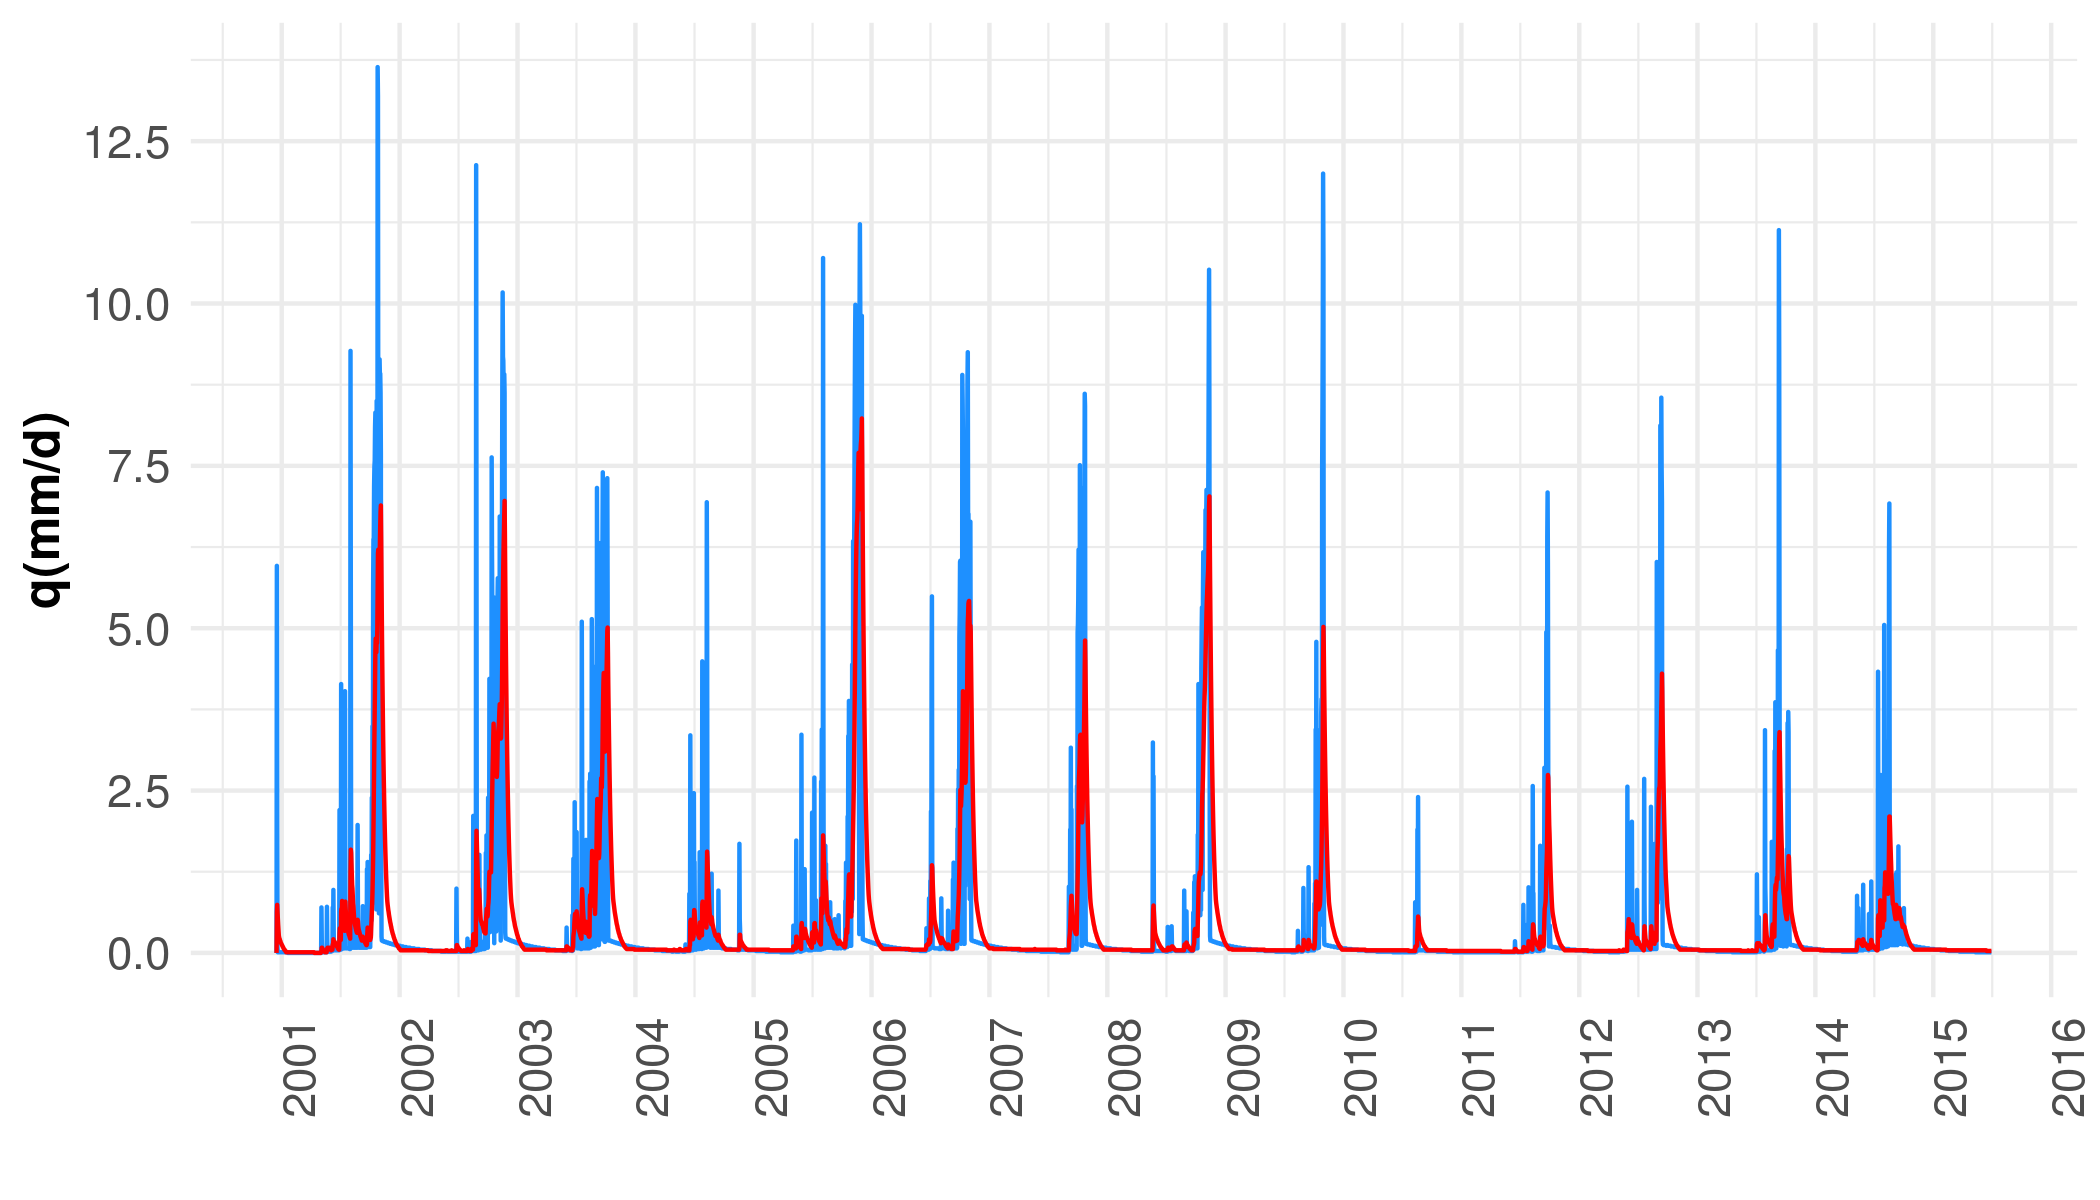
\includegraphics[scale = 0.8]{lumped_model}
  \caption{Observed (red) and simulated (blue) basin discharge. Note that the simulation does not precisely 
  reproduce the observed basin discharge, suggesting that the model needs some calibration.}
  \label{fig:lumped_model}
\end{figure}

It is required to manually change the \code{Routing{\_}HBV} parameters to approximate the simulation to the observed basin
discharge. Users will find in the package vignette (\code{vignette("lumped{\_}basin")}) more information on this example,
including the construction of an HBV model as a function and how to run a sensitivity analysis.


\subsection{Semi-distributed glacier mass balance}

In mountain areas with scarce meteorological information, temperature index models are widely used to simulate snow 
and ice melting \citep{hock:2003, konz:2010, finger:2015, ayala:2017}. Since air temperature is the most readily available
meteorological data in remote areas, the temperature index approach has been widely used in glaciological and hydrological
modeling \citep{ohmura:2001}. This package has been built with the \code{SnowGlacier{\_}HBV} function, a module that uses
this empirical approach to simulate snow, clean ice, and debris-covered melting.

In this section, we simulate the glacier mass balance for the Alerce glacier. Located on Monte Tronador ($41.15$º S ; $71.88$º W),
nearby the border between Argentina and Chile in the Andes of Northern Patagonia, Alerce is a medium-size mountain glacier 
with an area of about $2.33 \, km^2$ that ranges between $1629$ and $2358$ masl showing a SE aspect 
\citep{ruiz:2017, ingmanso:2018}.

\begin{figure}[htbp]
  \centering
  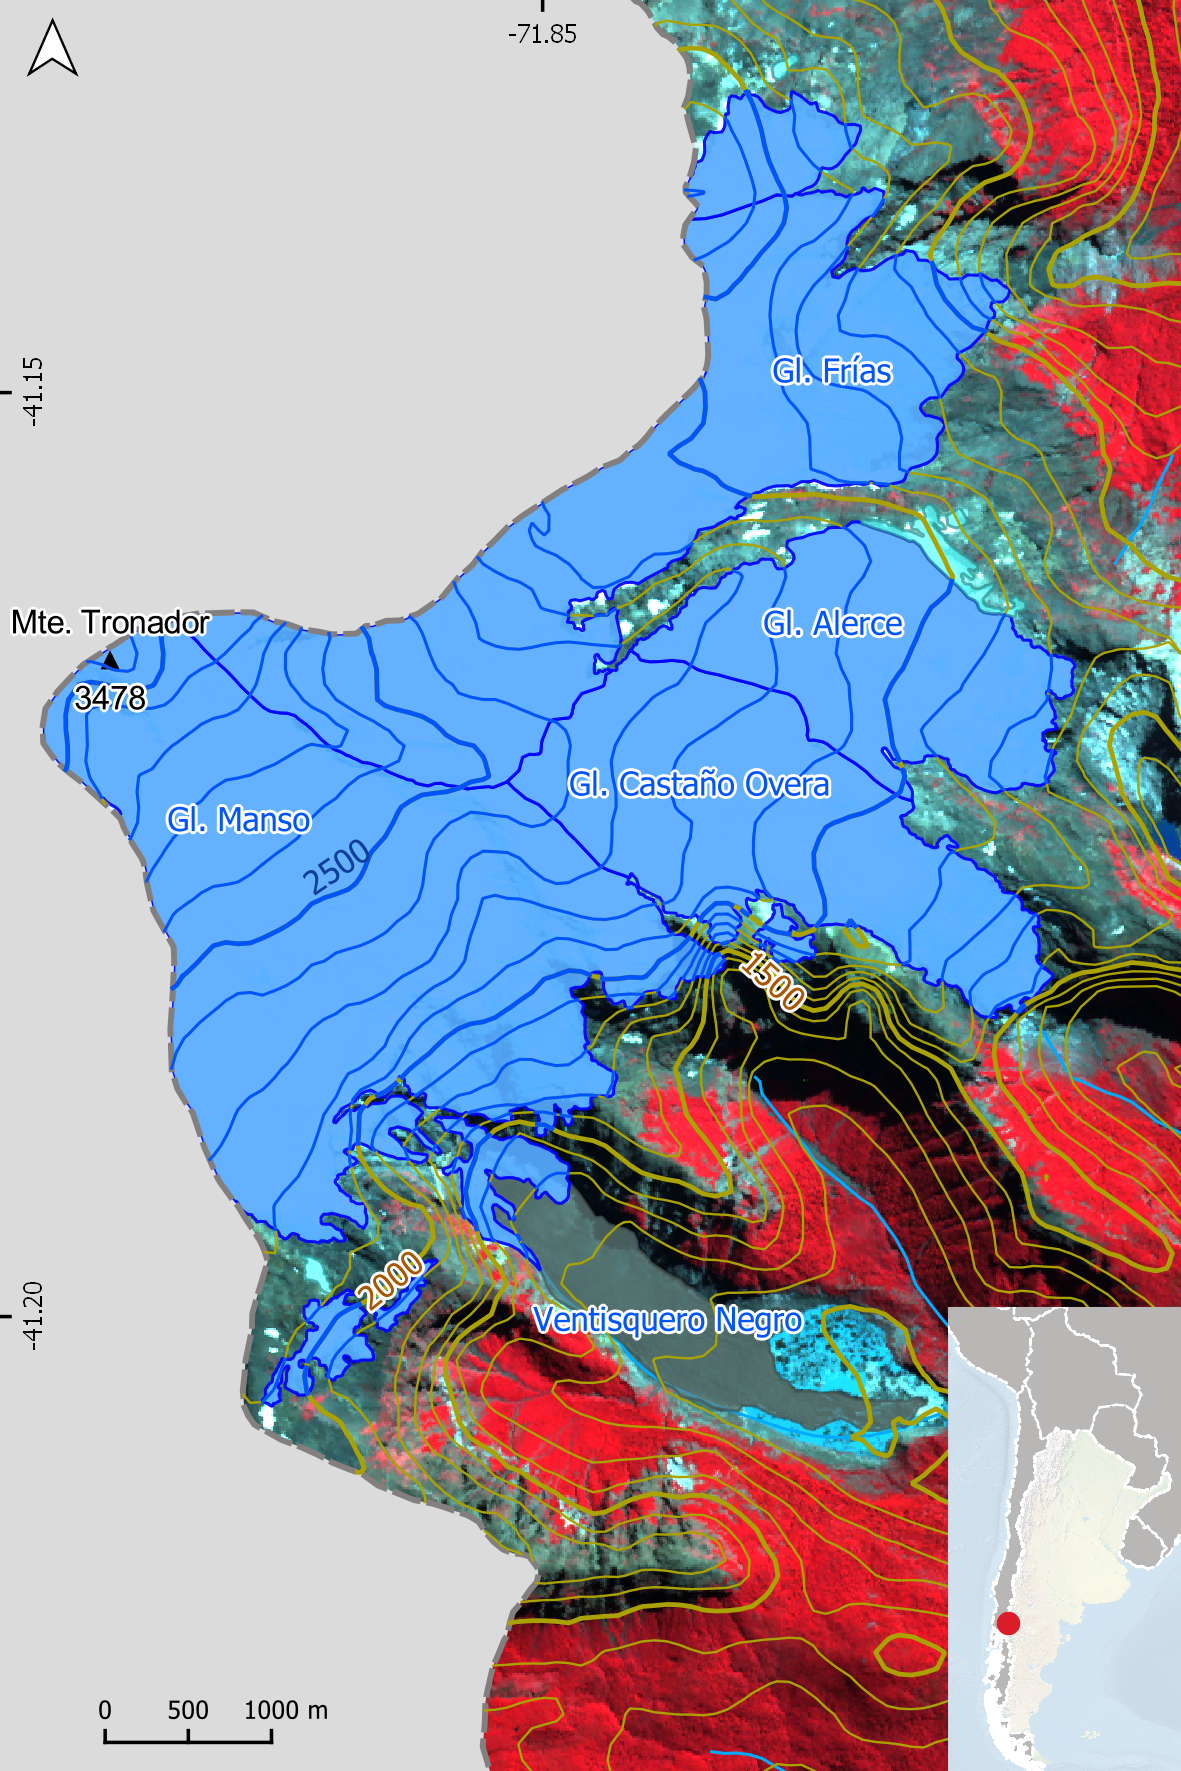
\includegraphics[scale = 0.6]{alerce_map}
  \caption{Satellite image of the Monte Tronador showing the location of the main glaciers. The Alerce
  glacier, located in the eastern sector, is one of the smallest glaciers at Monte Tronador.}
  \label{fig:alerce_map}
\end{figure}

Since $2013$, the Alerce glacier has been part of the monitoring network of the \textit{National Glacier Inventory}
\citep{ing_fundamentos:2010}. Measurements are conducted following the glaciological method for seasonal mass balance
computation \citep{kaser_manual:2003}. Puerto Montt precipitation (\textit{Dirección General de Aguas, Chile}) 
and Bariloche air temperature (\textit{Servicio Meteorológico Nacional - Argentina}) were used as meteorological 
records to simulate the annual mass balance of the glacier (\code{data(alerce{\_}data)}).\\
When calibrating the model parameters, simulations showing an annual mass balance in the range of $MB \pm 400 \, mm$ were
considered acceptable. $MB$ is the annual surface mass balance of the glacier.

\begin{example}
## load the dataset
data(alerce_data)

  # now extract 
    meteo_data   <- alerce_data[["meteo_data"]]   # meteorological forcing series
    mass_balance <- alerce_data[["mass_balance"]] # annual glacier mass balances
    mb_dates     <- alerce_data[["mb_dates"]]     # fix seasonal dates
    gl_topo      <- alerce_data[["topography"]]   # elevation bands
    
    z_tair   <- alerce_data[["station_height"]][1] # topo. elev. air temp.
    z_precip <- alerce_data[["station_height"]][2] # topo. elev. precip.
\end{example}

To evaluate the topographic effect on surface mass balance (derived from field measurements), the glacier was discretized into
elevation bands. To solve this problem, a semi-distributed glacier surface mass balance model (\code{glacier{\_}hbv}), 
an aggregation function (\code{agg{\_}mb} - since measurements and simulations are on different temporal scales), 
and a goodness-of-fit function (\code{my{\_}gof}) were constructed. The definition of this functions are included in
\code{vignette("alerce{\_}mass{\_}balance")}.

In the following code lines, the sampling strategy for finding acceptable parameter sets is indicated.

\begin{example}
# air temperature model
tair_range <- rbind(
  t_grad  = c(-9.8, -2)
)

# precip model
precip_range <- rbind(
  p_grad  = c(5, 25)
)

# glacier module
glacier_range <- rbind(
  sfcf = c(1, 2),
  tr   = c(0, 3),
  tt   = c(0, 3),
  fm   = c(1, 4),
  fi   = c(4, 8)
)

## aggregate them in a matrix
param_range <-
  rbind(
    tair_range,
    precip_range,
    glacier_range
  )
\end{example}

In the next step, we generate the random parameter sets:

\begin{example}
# set the number of model runs that you want to try
n_run <- 10000

# build the matrix
n_it <- nrow(param_range)

param_sets <- matrix(NA_real_, nrow = n_run, ncol = n_it)

colnames(param_sets) <- rownames(param_range)

set.seed(123) # just for reproducibility 
for(i in 1:n_it){

  param_sets[ , i] <- runif(n = n_run,
                            min = param_range[i, 1],
                            max = param_range[i, 2]
  )

}
\end{example}

Now, we combine the functions and extract our best simulations.

\begin{example}
# goodness of fit vector
gof <- c()

# make a loop
for(i in 1:n_run){

  # run the model
  glacier_sim <- glacier_hbv(topography = gl_topo,
                             meteo = meteo_data,
                             z_topo = c(z_tair, z_precip),
                             param_tair = param_sets[i, rownames(tair_range)],
                             param_precip = param_sets[i, rownames(precip_range) ],
                             param_ice = param_sets[i, rownames(glacier_range)] )

  # aggregate the simulation
  annual_mb <- agg_mb(x = glacier_sim,
                      start_date = as.Date( mb_dates$winter[-4] ),
                      end_date = as.Date( mb_dates$winter[-1] ) - 1 )

  # compare the simulations with measurements
  gof[i] <- my_gof(obs_upp = mass_balance$upp,
                   obs_lwr = mass_balance$lwr,
                   sim = annual_mb[ , 3])

  rm(glacier_sim, annual_mb)
}

param_sets <- cbind(param_sets, gof)

# we apply a filter
param_subset <- subset(x = param_sets, subset = gof == 3)
\end{example}

Once we have the subsetted our parameter matrix, we run the simulations to obtain a mean value (one per year).

\begin{example}
# now we run the model again to get our simulations
n_it <- nrow(param_subset)

mb_sim <- matrix(NA_real_, nrow = 3, ncol = n_it)

for(i in 1:n_it){
  glacier_sim <- glacier_hbv(topography = gl_topo,
                             meteo = meteo_data,
                             z_topo = c(z_tair, z_precip),
                             param_tair = param_subset[i, rownames(tair_range)],
                             param_precip = param_subset[i, rownames(precip_range) ],
                             param_ice = param_subset[i, rownames(glacier_range)] )

  annual_mb <- agg_mb(x = glacier_sim,
                      start_date = as.Date( mb_dates$winter[-4] ),
                      end_date = as.Date( mb_dates$winter[-1] ) - 1 )

  mb_sim[ , i] <- annual_mb[ , 3]

  rm(i, glacier_sim, annual_mb)

}

# now we are going to make a data frame with the mean surface mass balance simulation
mean_sim <- cbind( mass_balance,
                   "mb_sim" =  rowMeans(mb_sim)    )

# make the plot
library(ggplot2)
g1 <-
  ggplot(data =  mean_sim, aes(x = year)) +
  geom_pointrange(aes(y = `mb(mm we)`, ymin = `lwr`, color = 'obs',
                      ymax = `upp` ), size = 1,  fill = "white", shape = 21) +
  geom_point(aes(y = `mb_sim`, fill = 'sim'), shape = 23,
             size = 3) +
  geom_hline(yintercept = 0) +
  scale_y_continuous(limits = c(-1500, 500), breaks = seq(-1500, 500, 250) ) +
  scale_color_manual(name = '', values = c('obs' = 'blue') ) +
  scale_fill_manual(name = '', values = c('sim' = 'red') ) +
  ggtitle('') +
  xlab('') + ylab('mb (mm we)') +
  theme_minimal() +
  theme(
    title = element_text(color = "black", size = 12, face = "bold"),
    axis.title.x = element_text(color = "black", size = 12, face = "bold"),
    axis.title.y = element_text(color = "black", size = 12, face = "bold"),
    legend.text = element_text(size = 11),
    axis.text = element_text(size = 11))
\end{example}

\begin{figure}[htbp]
  \centering
  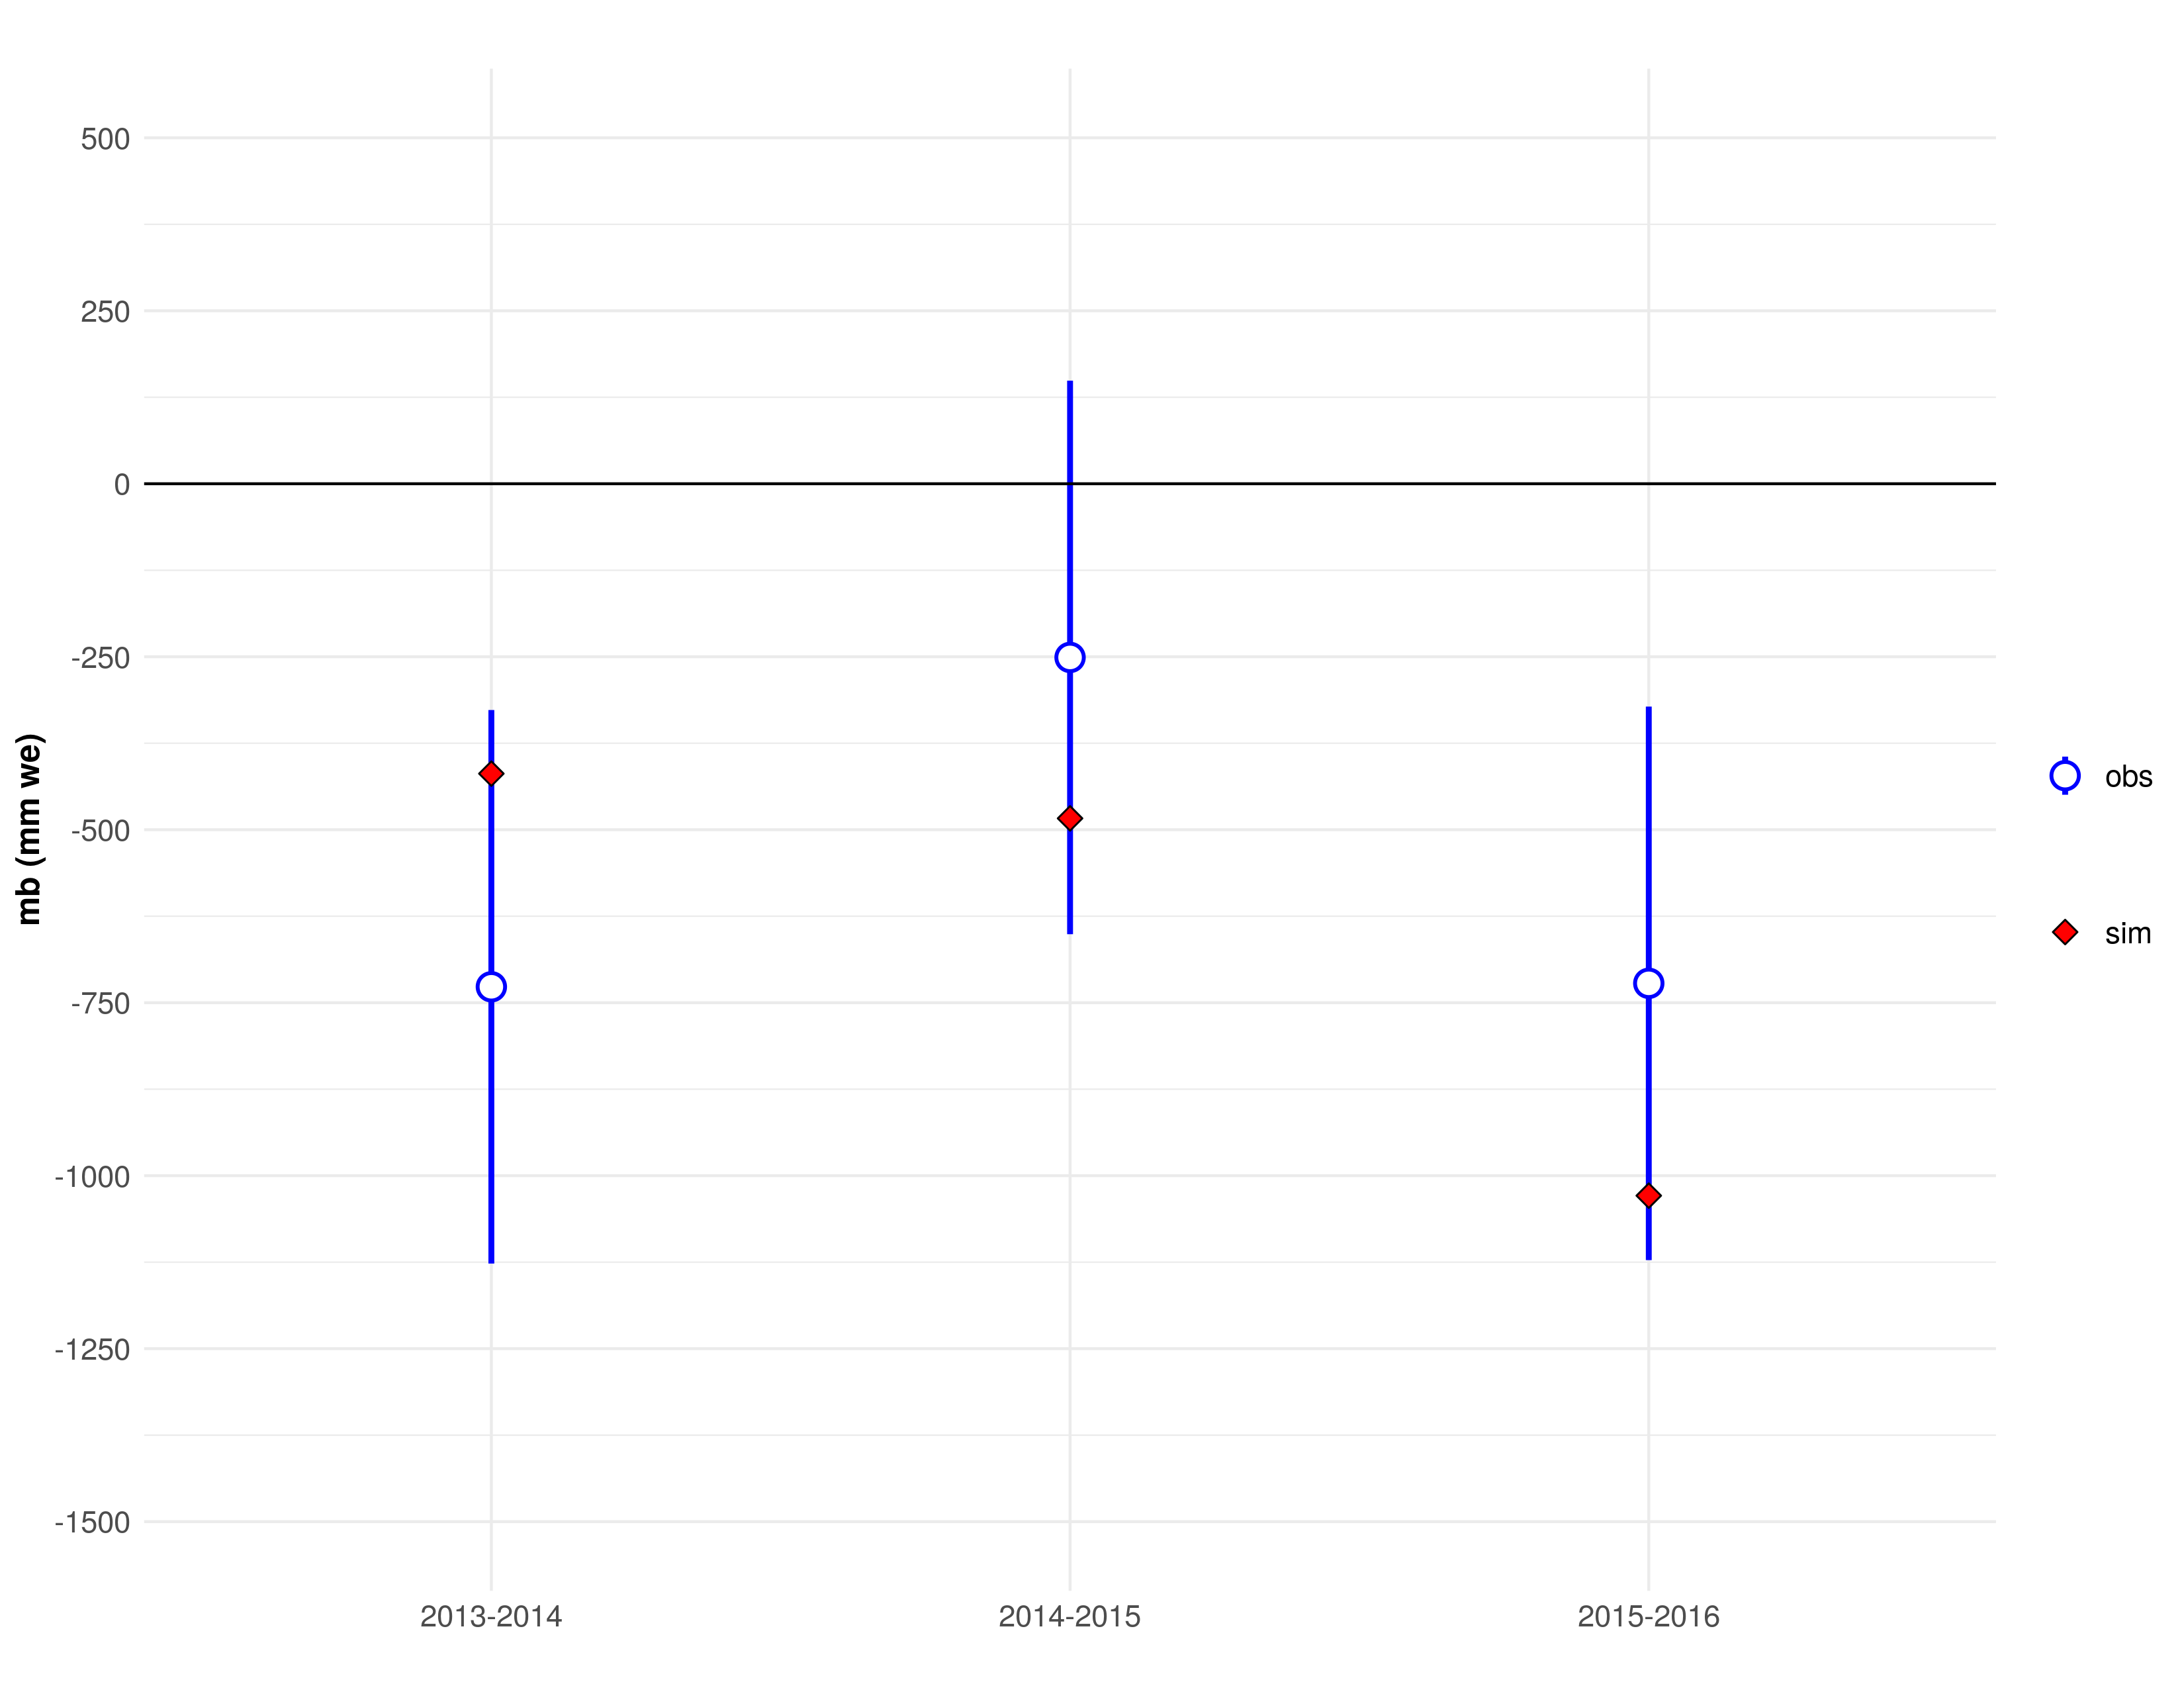
\includegraphics[scale = 0.5]{alerce_mass_balance}
  \caption{Annual mass balances for the period April 2013 - March 2016. All acceptable simulations lies between the 
  observed uncertainty bounds (despite the fact that we have plot just the mean value).}
  \label{fig:alerce_mb}
\end{figure}

\section{Summary}

In this study, we present the \pkg{HBV.IANIGLA} package, a modular version of HBV hydrological model that incorporates routines
for clean and debris-covered glacier modeling. We explain its modeling principles and philosophy; address the package modules and
related equations; and reinforce the importance of C++ code to speed up calculations, a characteristic that facilitates 
sensitivity and uncertainty analysis. To our knowledge, this is the first freely available, open-source modular version of the 
HBV model that incorporates routines for glacier surface mass balance modeling (clean and debris-covered ice).

We present two examples. The first one consists of a synthetic case to show how to build a model. This is the simplest
hydrological modeling case and should be use to understand how to concatenate the package functions and how a numerical
hydrological model works. The \code{vignette("lumped{\_}basin")} also illustrates the importance of sensitivity analysis and 
shows how it can be easily done in R. In fact, any kind of sensitivity or uncertainty analysis \citep{pianosi:2016} could be
incorporated into \pkg{HBV.IANIGLA}.
The second example, a real-world glacier surface mass balance estimation, was selected to show the use of the glacier module in
a semi-distributed case. This module could be of interest to the glaciological community, extending the use of the R language to
other scientific communities.

The new package version (0.2.1) documentation has been greatly improved in relation to previous versions, not only by clarifying
some aspects of the existing function’s documentation but also by adding six vignettes with reproducible examples (see
vignette(package = "HBV.IANIGLA")).

The modular design of the package allows the use of various spatio-temporal scales with dissimilar objectives in the same
environment (e.g., real-time streamflow forecasting, hydrological model teaching, or glacier mass balance simulation). 
The different modules can be combined with other R-related hydrological packages (e.g., \pkg{Evapotranspiration}, \pkg{DEoptim},
\pkg{topmodel}) or functions \citep{evap:2019, de_opt:2016, topmodel:2018}.

\pkg{HBV.IANIGLA} can also be combined with packages such as \CRANpkg{tidyverse}, \CRANpkg{sp}, \CRANpkg{raster},
\CRANpkg{hydroGOF}, or \CRANpkg{plotly} to build a single environmental hydrological workflow 
\citep{tidyverse:2019, sp:2017, raster:2017, hydroGOF:2017, plotly:2019}. Thus, a hydrological project can be developed from the
beginning to the end in the R environment, facilitating reproducible and repeatable research \citep{hutton:2016, ceola:2015}.
This type of model design opens up the possibility for applications beyond the Andes region as well as to incorporate new
functions, such as modules, to explicitly considering the dynamics of glaciers \citep{huss:2010}.

The package functions were built under generic classes (numeric vectors and matrices). This is an aspect where future 
improvements can be made. Since \pkg{HBV.IANIGLA} is available in modules, it could be greatly enhanced using 
the object-oriented programming (OOP) paradigm. In doing so, the model could represent an object with properties (e.g., areas,
polygons, elevations, among others), and the HBV routines as part of the methods (functional OOP - S4 types). These methods may
also include (but not limited to): sensitivity and uncertainty analysis, automatic plotting of results, and temporal aggregation
functionality. Even some methods could be recycled from the \CRANpkg{hydroToolkit} OOP package \citep{toum:2020}.

The package could also be improved by adding some GUI functionality keeping in mind that in the
words of \citet{chambers:2017}, \textit{...extending R is about contributing to the language through applications designed 
for a wider audience than the package author itself. Moreover, this objective should not be a target by its own, but a 
part or a piece of a bigger project directed to solve real world problems}.


\section{Acknowledgements}

E.T. acknowledges support from CONICET Argentina through a full-time PhD scholarship. The constructive suggestions from two
anonymous reviewers were very useful for improving the article, the package documentation, and the vignettes, and are greatly
appreciated. 


\bibliography{toum}

\address{Ezequiel Toum\\
  IANIGLA-CONICET\\
  Av. Ruiz Leal s/n Parque General San Martin - Mendoza\\
  Argentina\\
  %(ORCiD if desired)\\
  \email{etoum@mendoza-conicet.gob.ar}}
 
\address{Mariano H. Masiokas\\
  IANIGLA-CONICET\\
  Av. Ruiz Leal s/n Parque General San Martin - Mendoza\\
  Argentina\\
  %(ORCiD if desired)\\
  \email{mmasiokas@mendoza-conicet.gob.ar}}

\address{Ricardo Villalba\\
  IANIGLA-CONICET\\
  Av. Ruiz Leal s/n Parque General San Martin - Mendoza\\
  Argentina\\
  %(ORCiD if desired)\\
  \email{ricardo@mendoza-conicet.gob.ar}}
    
\address{Pierre Pitte\\
  IANIGLA-CONICET\\
  Av. Ruiz Leal s/n Parque General San Martin - Mendoza\\
  Argentina\\
  %(ORCiD if desired)\\
  \email{pierrepitte@mendoza-conicet.gob.ar}}
  
\address{Lucas Ruiz\\
  IANIGLA-CONICET\\
  Av. Ruiz Leal s/n Parque General San Martin - Mendoza\\
  Argentina\\
  %(ORCiD if desired)\\
  \email{lruiz@mendoza-conicet.gob.ar}}
